\documentclass[handout]{beamer}
%\documentclass[xcolor=pst]{beamer}
%\usepackage[spanish]{babel}
\usepackage[utf8x]{inputenc}

\usepackage{amssymb,amsmath}
\usepackage{graphicx} 
%\usepackage[pdf]{pstricks}
\usepackage{colortbl}
\definecolor{fucsia}{rgb}{1,0,1}
\usepackage[Q=yes]{examplep}

\newcounter{savedenum}
\newcommand*{\saveenum}{\setcounter{savedenum}{\theenumi}}
\newcommand*{\resume}{\setcounter{enumi}{\thesavedenum}}

%\usepackage{default}
\usetheme{Warsaw}

%\setbeamertemplate{caption}[numbered]


\title[Scatterplot clustering]{Scatterplot clustering for the integrative analysis of expression and methylation data}
%\author[shortname]{author1 \inst{1} \and author2 \inst{2}}
%\institute[shortinst]{\inst{1} affiliation for author1 \and 
%                      \inst{2} affiliation for author2}
\author[Ruiz de Villa]{M. Carme Ruiz de Villa, Francesc Carmona \\ Diego Arango del Corro, Josep Lluís Mosquera 
\\ Alex Sánchez}
\date[2013-05-23]{Mai 23, 2013}

\begin{document}
\begin{frame}
\begin{scriptsize}
\begin{center}
   XIV Conferencia Española de Biometría
\end{center}
\end{scriptsize}

\titlepage

\begin{columns}
   \column{0.7\textwidth}
   \scriptsize
   Departamento de Estadística \\ \textbf{Facultad de Biología}
    
   \hfill\column{0.3\textwidth}
   \includegraphics[height=1.25cm]{images/ub_marca_1l_pos_2t.pdf}
   %
\includegraphics[height=1cm]{images/ub-logo.jpg} 
\end{columns}
\end{frame}


\begin{frame}
\frametitle{Table of Contents}
\tableofcontents
\end{frame}

%\begin{frame}{La frase}
%\begin{center}
%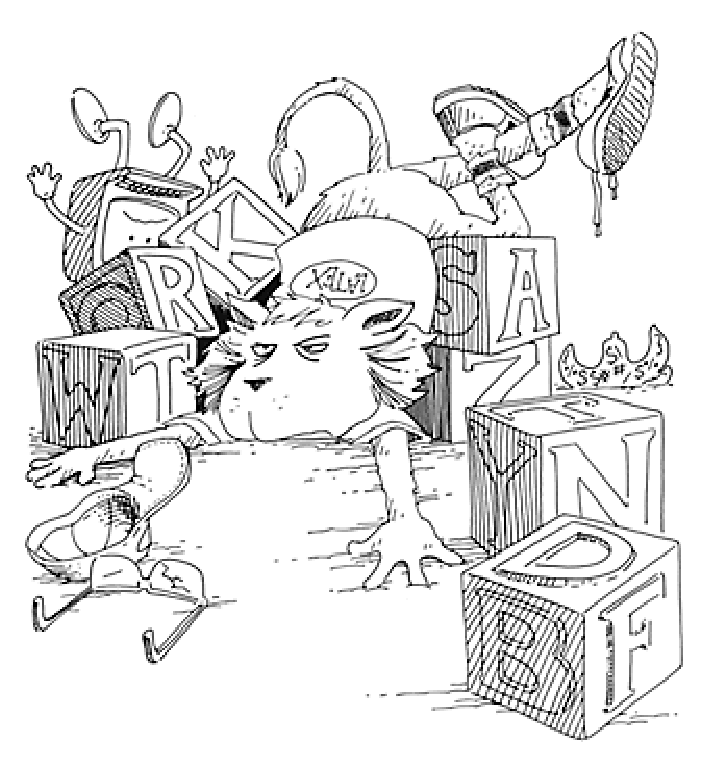
\includegraphics[height=5cm]{images/latex1.pdf}
%\end{center}
%\begin{center}
%\textbf{``Latex Allergy Cured by knitr''} 
%\end{center}
%\hfill Timely Portfolio
%\end{frame}

\begin{frame}{Objetivos}
\begin{block}{El objetivo principal}
El objetivo es
\begin{itemize}
\item primero
\item segundo
\item los resultados 
\end{itemize}
y todo funciona. 
\end{block}
\end{frame}

\section{Métodos estadísticos}

\subsection{Gene-specific methylation on-off threshold}

\begin{frame}{}
Methylation is often described as a binary on-off signal,
and it is widely recognized that methylation represses gene
expression. Typically, if a gene is controlled by its methylation,
its expression is low when methylated. 
On the other hand,
when unmethylated, its expression can be either high or low.
Since measurements for methylation and expression are both
continuous, a biaxial plot of these two signals will exhibit an
L-shape pattern. 

If we truly
believe that methylation is binary, there are two implications:
\begin{enumerate}
\item the reflection point of the L-shape is an appropriate choice
to binarize methylation data, and
\item conditioning on the
binarized on-off methylation status, the continuous valued
methylation data and expression data should be independent,
\end{enumerate}
which motivates Liu(2012) to quantify the L-shape pattern using
conditional mutual information (MI). 

%In this section, we
%use TCGA data to ask 

\end{frame}

\begin{frame}{Conditional Mutual Information}
Two questions: which genes exhibit
L-shape, and what is the optimal threshold for binarizing
methylation data for each L-shape gene.
\begin{block}{The key}
To determine whether methylation and expression of a gene exhibit an L-shape,
we compute the conditional Mutual Information (MI) for different choices of threshold
to binarize the methylation data.
\end{block}
If we consider the continuous valued methylation and expression data as two random variables
$X$ and $Y$, and denote a nominal threshold as $t$, the conditional MI can be written as a
weighted sum of MIs on the two sides of the threshold.
\[
\mathit{cMI}(t)=I(X,Y|X>t)P(X>t) + I(X,Y|X\le t)P(X\le t)
\]
\end{frame}

\begin{frame}{Optimal threshold}
When $t$ is $0$ or $1$, $\mathit{cMI}$ equals to the mutual information derived 
from all data points.

For an L-shape gene, as $t$ moves from 0 to 1, $\mathit{cMI}(t)$ first decreases and then
increases, and its value approaches zero when $t$ coincides with the reflection point. 
Therefore,
\begin{block}{Optimal threshold}
The ratio $r=\frac{\min\{\mathit{cMI}(t)\}}{\mathit{cMI}(0)}$ for an L-shape gene is small, 
and $t^{\ast} = \mathrm{argmin}\{ \mathit{cMI}(t) \}$ is the optimal threshold for 
dichotomizing the methylation data of this gene.
\end{block}

\end{frame}

\begin{frame}{Joint distribution estimator}
To estimate the MI terms we use a kernel-based estimator, which constructs a joint
probability distribution by applying a Gaussian kernel to each data point, and estimates
the MI based on the joint distribution. The estimator is as follows:
\[
I(X,Y) = \frac 1M \sum_{i=1}^M \log\frac{M\sum_{j=1}^M e^{-\frac{1}{2h^2}((x_i-x_j)^2+(y_i-y_j)^2)}}{%
                                      \sum_{j=1}^M e^{-\frac{1}{2h^2}(x_i-x_j)^2} \sum_{j=1}^M e^{-\frac{1}{2h^2}(y_i-y_j)^2}}
\]
where $h$ is a tuning parameter for the kernel width and empirically set $h=0.3$.
% i and j are indices for samples.
% In our analysis, we normalize the expression data to zero mean.
\end{frame}

\begin{frame}{L-shapes}
\begin{block}{Three criteria}
We filtered for L-shapes using a combination of three criteria:
\begin{itemize}
\item the ratio $r<0.25$
\item unconditioned MI $\mathit{cMI}(0)>0.1$
\item the median expression on the left side of the optimal threshold $t^{\ast}$ is higher
than the median expression on the right side.
\end{itemize}
\end{block}
The parameters are chosen according to a random permutation test (see Liu(2012)).

According to the above criteria, a total of 641 genes are selected to be L-shape genes.
\end{frame}

\begin{frame}{Clustering using Spline regression }
We implemented regression based on  \textit{$B$-splines} because they are particularly efficient due to the block-diagonal basis matrices that result.

Let 
\begin {itemize}
\item $\varsigma=\lbrace t_1 < \ldots < t_N \rbrace$ non decreasing  knot sequence 
\item $\left[ t_m,t_{m+1} \right)$ half open interval
\item $B_{mp}$ $p$-th order polynomial (degree $p-1$) with finite support over the interval and 0 everywhere else so that  $\sum_{m=1}^{N-p}B_{mp}(x)=1$
\item then  $s(x)=\sum_{m=1}^{N-p}B_{mp}(x)c_m$ 
\end{itemize}
\end{frame}

\begin{frame}{Clustering using Spline regression (2)}
To represent the curve we set:
\[
y_{ij}=s_{ij}
\]
So
\[ 
\mathbf{y}_i=\mathbf{B}_i\mathbf{c}
\]
with
\begin {itemize}
\item $\mathbf{B}_i=\left[ B_{1p}\mathbf{x}_i,B_{2p}\mathbf{x}_i,\dots,B_{Lp}\mathbf{x}_i \right]$ the spline basis matrix
\item $\mathbf{c}$ the vector of spline coefficients.
\end{itemize}
\end{frame}

\begin{frame}{Clustering using Spline regression (3)}
Analysis
\begin {itemize}
\item Selection of the genes with a negative significant correlation
\item Fit cubic regression splines
\item Data to cluster: splines coefficients
\item Calculation of a distance matrix between genes as $1-\rho$
\item Hierarchical clustering 
\end{itemize}
\end{frame}

\begin {frame}{Results}
\textbf{Hierarchical clustering}:
\begin {itemize}
\item After the previous selection of genes we worked with 292 genes
\item We decided to choose 5 clusters
\item The 2 first clusters included the genes with an L-shape
\end{itemize}
\textbf{Mutual Information}
\begin{itemize}
\item No previous selection of the genes was needed
\end{itemize}
We have found similar results between both methods that can be summarized in the following table:
\begin{center}
\begin{tabular}{|c|c|c|}
\hline
Cluster & Splines & cMI \\
\hline
1 & 140 & 102 \\
2 & 22 & 16 \\
\hline
Total & 162 & 118 \\
\hline
\end{tabular}
\end{center}
\end{frame}

%\begin {frame}{Graphics}
%\begin{center}
%\includegraphics[height=5cm]{images/Plot1.pdf}
%\end{center}
%\begin{center}
%\textbf{``           ''} 
%\end{center}
%\hfill Timely Portfolio
%\end{frame}


\end{document}
